\section{Experimental Design}
The null hypothesis for this experiment are:
\begin{enumerate}
  \item k-NN is not the most accurate machine learning model to classify 18 Metal subgenres.
  \item There is not more than 40\% confusion between two subgenres over at least two classifiers.
\end{enumerate}


To test for the hypotheses, the same models, hyperparameters and features will be used as \textit{Phase C} by Ndou et al. \cite{ndou2021music}. A new dataset is created for this experiment. This dataset contains 1800 tracks. For each subgenre, the most popular public Spotify playlist with at least 100 tracks found on 2024/11/20 is used. After compiling the tracks, the features as described by Table~\ref{tab:feature_rep_dims} are extracted. For each track, 9 slices are taken. This is because \verb|librosa| calculates the last slice to be around 2.7 seconds so it is discarded for being too short. The tracks were not downloaded to disk due to copyright and ethical concerns. Instead, Python's \verb|io.BytesIO| handles them directly in memory. Additionally, Spotify rate limits the API, hence the feature extraction process had to be split into two spaced apart sessions. One final deterrent is that some tracks are unavailable to the UK market \cite{eriksson2019spotify} so the final dataset has 14,572 slices.

\begin{table}[h!]
\centering
\begin{tabular}{|l|c|}
\hline
\textbf{Classifier} & \textbf{Hyperparameters} \\ \hline
k-Nearest Neighbours & nearest neighbours=1 \\ \hline
Multilayer Perceptron & activation=ReLu, solver=lbfgs \\ \hline
Random Forests & number of trees=1000, max depth=10, \\ 
& $\alpha = e^{-5}$, hidden layer sizes=(5000,10) \\ \hline
Support Vector Machines & decision function shape=ovo \\ \hline
Logistic Regression & penalty=12, multi class=multinomial \\ \hline
\end{tabular}
\caption{Classifier Hyperparameters}
\label{tab:classifier_hyperparams}
\end{table}

\begin{table}[h!]
\centering
\begin{tabular}{|l|c|c|}
\hline
\textbf{Features} & \textbf{Representation} \\ \hline
Chroma                     & Mean + SD\textsuperscript{2}  \\ \hline
Root Mean Square           & Mean + SD\textsuperscript{2}  \\ \hline
Spectral Centroid          & Mean + SD\textsuperscript{2}  \\ \hline
Spectral Bandwidth         & Mean + SD\textsuperscript{2}  \\ \hline
Spectral Rolloff           & Mean + SD\textsuperscript{2}  \\ \hline
Zero Crossing Rate         & Mean + SD\textsuperscript{2} \\ \hline
Mel Frequency Cepstral Coefficients & Mean + SD\textsuperscript{2}\\ \hline
Harmony                    & Mean + SD\textsuperscript{2} \\ \hline
Tempo                      & Mean                         \\ \hline
\end{tabular}
\caption{Feature Representation}
\label{tab:feature_rep_dims}
\end{table}

Each of the above classifiers were evaluated using stratified 3-repeated 10-fold cross validation. As per \href{https://scikit-learn.org/dev/modules/cross_validation.html#stratified-k-fold}{scikit-learn's documentation}, "Stratified k-fold is a variation of k-fold which returns stratified folds: each set contains approximately the same percentage of samples of each target class as the complete set." This results in 30 runs per classifier with the same train and test splits, in which the accuracy and F1 scores are calculated. For the second hypothesis, the confusion of each classifier is calculated as a mean due to the stratified nature of the folds.

For statistical significance, Shapiro-Wilk test is done on the accuracies to check for normal distribution. if so, a one-way ANOVA accompanied by a pairwise Tukey HSD will look into all comparisons involving k-NN, and show which model is more significantly accurate. For the second hypothesis, a qualitativer approach will count the amount of classifiers that confuse a pair of subgenres is at least two.

\begin{figure}[h!]
    \centering
    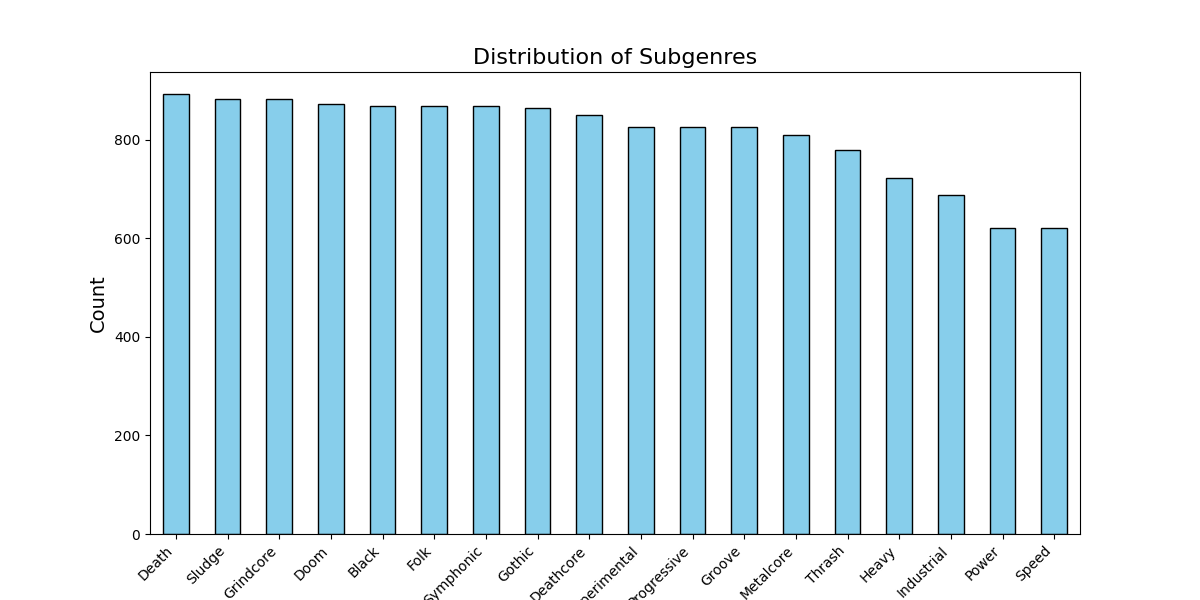
\includegraphics[width=\textwidth]{figures/subgenre_distribution.png} 
    \caption{Subgenres are not evenly distributed due unavailability in the UK}
    \label{fig:dist}
\end{figure}
